
\documentclass{article}
\usepackage{amsmath}
\usepackage[margin=1in]{geometry}
\usepackage{amsfonts}
\usepackage{hyperref}
\usepackage{graphicx}
\usepackage{siunitx}
\usepackage{cancel}
\usepackage{xfrac}


\begin{document}
	
	\title{Change of Variables}
	\author{Andy Chong Sam}
	\date{}
	\maketitle
	
	\section{Overview}
	
	\par\noindent If there is a transformation that translates from a \((u,v)\) coordinate system to the standard \((x,y)\) system then we can use the Jacobian to integrate in the \((u,v)\) system instead. We would want to do this if integrating on \((u,v)\) is less calculation intensive than on \((x,y)\). 
	
	\section{Deriving the Jacobian}
	
	\par\noindent In Figure 1 we have a transformation \(T\) which maps from \((u,v)\) to \((x,y)\). Using linear algebra terms, the graph on the right is an image of the transformation. In this transformation, we have two hypothetical functions \(x = g(u,v)\) and \(y = h(u,v)\). We can summarize the transformation as a vector function \(r\).
	
	\begin{center}
		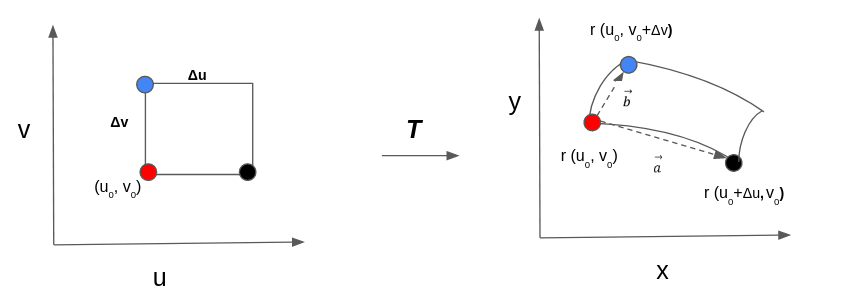
\includegraphics[width=9cm]{uvtoxymapping.png}\\
		Figure 1
	\end{center}
	
	\par \noindent From this same example we can derive the following two secant vectors:
	\begin{flalign*}
		\vec a = r(u_0+ \Delta v, v_0) - r(u_0,v_0) \\
		\vec b = r(u_0, v_0 + \Delta v) - r(u_0,v_0)
	\end{flalign*}
	
	\par\noindent If \(r\) describes the image on \((x,y)\) using \((u,v)\), then \(r_u\) and \(r_v\) are partial derivatives that measure the change in \(r\) with respect to \(u\) and \(v\).
	\begin{flalign*}
		r_u = g_u (u_0, v_0) \vec i + h_u (u_0, v_0)\vec j \\
		r_v = g_v (u_0, v_0) \vec i + h_v (u_0, v_0)\vec j
	\end{flalign*}

	\par\noindent We know that the formal definition of \(r_u\) is:
	
	\begin{flalign*}
		r_u = \lim_{\Delta \to 0}\frac{r(u_0 + \Delta u, v_0)-r(u_0,v_0)}{\Delta u}
	\end{flalign*}

	\par\noindent For small values \(\Delta u\) we can say that:
	
	\begin{flalign*}
		r_u \Delta u = r(u_0 + \Delta u, v_0)-r(u_0,v_0)
	\end{flalign*}
	\pagebreak

	\par\noindent 
	
		\begin{minipage}{.5\linewidth}		
		\par \noindent The vector \(r_u\Delta u\) serves as an approximation of \(\vec a\), and \(r_v\Delta v\) serves as an approximation of \(\vec b\). This is illustrated in Figure 2.
		\newline
		\par\noindent The cross product  \(\Delta u r_u \times \Delta v r_v\) forms a parallelogram that approximates the area covered as a result of extending from \((u_0,v_0)\) by the amounts of \(\Delta u\) and \(\Delta v\). If we simplify the cross product further:
			\begin{flalign*}
			|\;\Delta u r_u \times \Delta v r_v \;| = \Delta u \Delta v |r_u \times r_v |
		\end{flalign*}
		
	\end{minipage}
	\begin{minipage}[c]{.5\linewidth}
		
		\begin{center}
			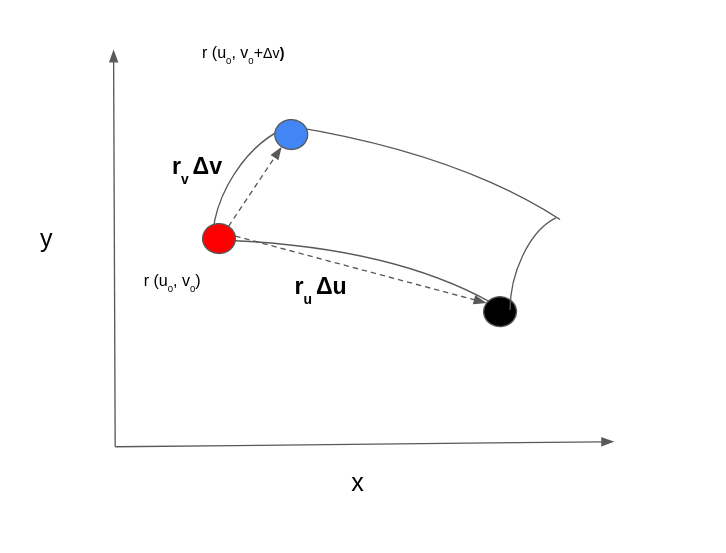
\includegraphics[width=7cm]{uvtoxymapping-1.png}
		\end{center}
		
		\begin{center}
			Figure 2
		\end{center}
		
	\end{minipage}
	\newline
	\newline
	\par\noindent The cross product \(r_u \times r_v\) can be obtained by calculating the following determinant:
	\newline
	\[
	det \left(\begin{array}{@{}cc@{}}
		\frac{\partial g}{\partial u} & \frac{\partial g}{\partial v} \\ \\ 
		\frac{\partial h}{\partial u} &  \frac{\partial h}{\partial v}
	\end{array}\right) = \frac{\partial g}{\partial u} \frac{\partial h}{\partial v} - \frac{\partial g}{\partial v}\frac{\partial h}{\partial u}
	\]
	\par\noindent Because \(g\) and \(h\) are just descriptions of the \(x\) and \(y\) coordinates in the transformation, we typically write this result as: 
	
	\begin{flalign}
		J = \frac{\partial (x,y)}{\partial (u,v)} = \frac{\partial x}{\partial u} \frac{\partial y}{\partial v} - \frac{\partial x}{\partial v}\frac{\partial y}{\partial u}
	\end{flalign}

	\par\noindent Expression (1) is the Jacobian.
	\newline
	\newline
	\begin{minipage}{.5\linewidth}		

	\par\noindent In Figure 3 we've squared off several regions of length \(\Delta u\) and \(\Delta v\). Let's suppose that the transformation maps these to the regions on the right on the \(xy\) plane. Let's label the surface on the right \(f\). The volume under a section of \(f\) is the double integral:
	
	\begin{flalign*}
		\int \int f(x,y)\; dA \approx \sum_{i=1}^{m}\;\sum_{i=1}^{n} f(x,y) \Delta A
	\end{flalign*}

\end{minipage}
\begin{minipage}[c]{.5\linewidth}
		\begin{center}
		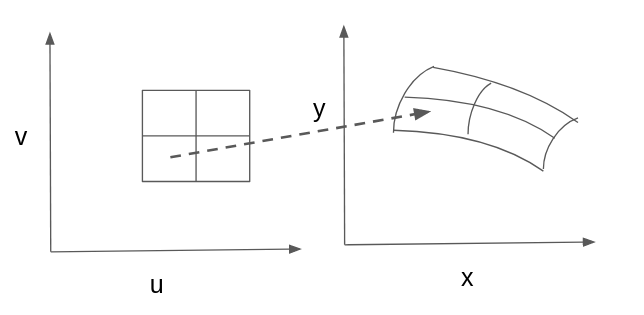
\includegraphics[width=6cm]{uvtoxymapping-2.png}
	\end{center}
	
	\begin{center}
		Figure 3
	\end{center}

	
\end{minipage}
\newline
\newline
\par\noindent In the previous section we saw how to approximate a region of \(f\) with the rectangle \(\Delta u \Delta v |r_u \times r_v |\;\;\). If we take infinitesimal measurements of \(\Delta u\) and \(\Delta v\), we get the following:

\begin{flalign*}
\sum_{i=1}^{m}\;\sum_{i=1}^{n} f(x,y) \Delta A = \sum_{i=1}^{m}\;\sum_{i=1}^{n} f(g(u,v),h(u,v))\; |\;\frac{\partial(x,y)}{\partial(u,v)}\;|\;\Delta u \;\Delta v
\end{flalign*}
\par\noindent With infinitesimal measurements for \(\Delta u\) and \(\Delta v\) we obtain the following double integral:

\begin{flalign}
	\int \int f( g(u,v), h(u,v) ) \; |\;\frac{\partial(x,y)}{\partial(u,v)}\;|\;du\;dv
\end{flalign}

\par\noindent Expression (2) represents the general methodology for how to apply change of variables to a double integral.
\newline
\newline
\framebox{
	\parbox{\linewidth}{
		\par \textbf{Ex. 1}	Evaluate \(\int\int_{R}(x-3y)\;dA\). \(R\) is defined as the parallelogram with points \((0,0)\), \((3,3)\), \((7,3)\), \((4,0)\). The following transformation can be used \(x=u+v\) and \(y=u\).
		\newline
	\par\noindent Source: Larson, Calculus 6th Edition, pg 1032
		\newline
		\par \noindent The parallelogram can be defined with four lines. We can apply the transformation to each of the lines:
		\begin{flalign*}
			\text{Line A:}\;\;\;\; y=0\;\;\;\;    \to \;\;\;\; u =0 \\
			\text{Line B:}\;\;\;\; y=x-4\;\;\;\; \to \;\;\;\; v = 4 \\
			\text{Line C:}\;\;\;\; y=3 \;\;\;\; \to \;\;\;\; u = 3 \\
			\text{Line D:}\;\;\;\; y=x \;\;\;\; \to \;\;\;\; v = 0
		\end{flalign*}
		\par \noindent The new area of intetegration will be a rectangle with the bounds \(0 \leq u \leq 3\) and \(0 \leq v \leq 4\).
		\newline
		\par\noindent We calculate the Jacobian and evaluate the integral:
		\[J=
		det \left(\begin{array}{@{}cc@{}}
			\frac{\partial x}{\partial u} & \frac{\partial x}{\partial v} \\ \\ 
			\frac{\partial y}{\partial u} &  \frac{\partial y}{\partial v}
		\end{array}\right) = 
		det \left(\begin{array}{@{}cc@{}}
			1 & 1 \\ \\ 
			1 & 0
		\end{array}\right) = -1
		\]
		\begin{flalign*}
			\int\int_{R}(x-3y)\;dA = \int_{0}^{3} \int_{0}^{4}\;uv\;|-1|\;dvdu = \int_{0}^{3} \int_{0}^{4}\;uv\;\;dvdu \\
			\int_{0}^{3}\;\frac{uv^2}{2} \Big|_0^4\;du = 8(\frac{u^2}{2} \Big|_0^3) = 36
		\end{flalign*}
}}
\newline
\newline
\newline
\framebox{
	\parbox{\linewidth}{
		\par \textbf{Ex. 2} Evaluate \(\int \int_{R}x-3y\;dA\). \(R\) is a region described by a triangle with the following points \((0,0)\), \((1,2)\), \((2,1)\). The following transformation is available: \(x=2u+v\) and \(y=u+2v\).
		\newline
		\par\noindent Source: Stewart, Calculus 8th Edition pg 1060
		\newline
		\par The triangle can be described with three lines. We apply the transformation to each of these:
		
		\begin{flalign*}
			\text{Line A:}\;\;\;\;y=\frac{1}{2}x\;\;\;\;\to\;\;\;\;v=0\\
			\text{Line B:}\;\;\;\;y=3-x\;\;\;\;\to\;\;\;\;v=1-u\\
			\text{Line C:}\;\;\;\;y=2x\;\;\;\;\to\;\;\;\;u=0 \\
		\end{flalign*}
	
		\par\noindent For Line B the u-intercept is \(1\). This combined with the transformations above give us the following bounds, \(0 \leq u \leq 1\), and \(0 \leq v \leq 1-u\).
		\newline 
		\par\noindent We calculate the Jacobian and evaluate the integral:
		\[J=
		det \left(\begin{array}{@{}cc@{}}
			\frac{\partial x}{\partial u} & \frac{\partial x}{\partial v} \\ \\ 
			\frac{\partial y}{\partial u} &  \frac{\partial y}{\partial v}
		\end{array}\right) = 
		det \left(\begin{array}{@{}cc@{}}
			2 & 1 \\ \\ 
			1 & 2
		\end{array}\right) = 3
		\]
		\begin{flalign*}
			\int \int_{R}x-3y\;dA = 3\int_{0}^{1}\int_{0}^{1-u}-u-5v\;dvdu \\	
			3\int_{0}^{1} -uv - \frac{5v^2}{2} \Big|_0^{1-u}\;du = \int_{0}^{1} = 3\int_{0}^{1} -u(1-u) - \frac{5}{2}(1-u)^2 = -3
		\end{flalign*}
}} 
\newpage
\section{Polar Coordinates}
\par\noindent The evaluation of double integrals using polar coordinates is an application of these techniques. We know that \(x=r\cos \theta\) and \(y=r\sin \theta\). If we compute the Jacobian:

		\[J=
det \left(\begin{array}{@{}cc@{}}
	\frac{\partial x}{\partial r} & \frac{\partial x}{\partial \theta} \\ \\ 
	\frac{\partial y}{\partial r} &  \frac{\partial y}{\partial \theta}
\end{array}\right) = 
det \left(\begin{array}{@{}cc@{}}
	\cos \theta & -r\sin \theta \\ \\ 
	\sin \theta  & r \cos \theta
\end{array}\right) = r(cos^2 \theta + sin^2 \theta) = r
\]
\par\noindent If we had a function \(f(x,y)\) and apply a change of variables:

\begin{flalign*}
	\int\int f(x,y)\;dydx = \int_{r=b}^{r=a}\int_{\theta=d}^{\theta=c}f(x(\theta, r), y(\theta, r)) r \;drd\theta
\end{flalign*}

\framebox{
	\parbox{\linewidth}{
	\par\noindent \textbf{Ex. 3} Evaluate \(\int \int_{R}x^2\;dA\). \(R\) is an ellipse, \(9x^2 + 4y^2=36\). The following transformation can be used \(x=2u\) and \(y=3v\).
	\newline
		\par\noindent Source: Stewart, Calculus 8th Edition pg 1060
	\newline
	\par\noindent Let's just try and plug in the transformation into \(R\), we get:
	\begin{flalign*}
		9(2u)^2 + 4(3v)^2 = 36 \\
		u^2 + v^2 = 1
	\end{flalign*}
	\par\noindent The transformation has given us a circle, which will be easier to integrate. Next, we figure out the Jacobian:
	
			\[J=
	det \left(\begin{array}{@{}cc@{}}
		\frac{\partial x}{\partial u} & \frac{\partial x}{\partial v} \\ \\ 
		\frac{\partial y}{\partial u} &  \frac{\partial y}{\partial v}
	\end{array}\right) = 
	det \left(\begin{array}{@{}cc@{}}
		2 & 0 \\ \\ 
		0 & 3
	\end{array}\right) = 6
	\]
	
	\par\noindent We are left with the following integral:
	
	\begin{flalign*}
		24 \int\int u^2\;dudv
	\end{flalign*}

	\par\noindent We can now apply another change of variables to polar coordinates to complete the integration:
	
	\begin{flalign*}
					24\int_{0}^{2 \pi} \int_{0}^{1} r^2 \cos^2 \theta\;r \;drd\theta
	\end{flalign*}
	
	\begin{flalign*}
			24\int_{0}^{2 \pi} \frac{r^4}{4} \cos ^2 \theta \Big|_0^{1} \; d \theta = 
			6\int_{0}^{2 \pi} \cos^2 \theta \;d\theta = 6(\frac{\theta}{2}+ \frac{\sin(2\theta)}{4})\Big|_0^{2\pi} = 6\pi \\
	\end{flalign*}
}}

\end{document}